% !TEX program = xelatex
\documentclass[11pt,a4paper,fontset=windows]{ctexart}
\usepackage[margin=2.2cm]{geometry}
\usepackage{amsmath,amssymb,amsthm,mathtools,bm}
\usepackage{graphicx}
\usepackage{booktabs,array,multirow,tabularx}
\usepackage[table]{xcolor}
\usepackage{caption}
\usepackage{enumitem}
\usepackage[most]{tcolorbox}
\usepackage[colorlinks=true,linkcolor=blue!55!black,citecolor=green!40!black,urlcolor=blue!55!black,
            pdftitle={黑洞 QNM 谱不稳定性与可观测振铃稳定性},pdfauthor={Claude (Opus 5.5)}]{hyperref}

\captionsetup{font=small,labelfont=bf}
\setlist{itemsep=2pt,topsep=3pt}
\ctexset{section/format=\Large\bfseries\raggedright}

% ---------------- status tags ----------------
\newcommand{\tagbox}[2]{\begingroup\setlength{\fboxsep}{1.4pt}\colorbox{#1}{\textcolor{white}{\footnotesize\bfseries #2}}\endgroup}
\newcommand{\proven}{\tagbox{green!45!black}{已证明}}
\newcommand{\sketch}{\tagbox{teal!80!black}{证明概要}}
\newcommand{\condJ}{\tagbox{blue!65!black}{已证明\,|\,条件 J}}
\newcommand{\condJa}{\tagbox{blue!65!black}{已证明\,|\,条件 J-asym}}
\newcommand{\exactlow}{\tagbox{violet!80!black}{精确低阶}}
\newcommand{\numer}{\tagbox{orange!85!black}{数值}}
\newcommand{\conj}{\tagbox{red!70!black}{猜想}}

% ---------------- theorem environments ----------------
\theoremstyle{definition}
\newtheorem{theorem}{定理}
\newtheorem{proposition}{命题}
\newtheorem{corollary}{推论}
\newtheorem{conjecture}{猜想}
\newtheorem{lemma}{引理}
\theoremstyle{definition}
\newtheorem{assumption}{假设}
\renewcommand{\proofname}{证明}
\renewcommand{\qedsymbol}{$\blacksquare$}

% ---------------- macros ----------------
\newcommand{\eps}{\varepsilon}
\newcommand{\cE}{\mathcal E}
\newcommand{\cM}{\mathcal M}
\newcommand{\cA}{\mathcal A}
\newcommand{\cW}{\mathcal W}
\newcommand{\cG}{\mathcal G}
\newcommand{\cR}{\mathcal R}
\newcommand{\cP}{\mathcal P}
\newcommand{\Ain}{A_{\rm in}}
\newcommand{\Aout}{A_{\rm out}}
\renewcommand{\Im}{\operatorname{Im}}
\renewcommand{\Re}{\operatorname{Re}}
\DeclareMathOperator{\supp}{supp}
\newcommand{\dd}{\mathrm d}
\newcommand{\tauS}{\tau_*}

\tcbset{keybox/.style={colback=blue!3,colframe=blue!45!black,boxrule=0.6pt,arc=2pt,left=6pt,right=6pt,top=4pt,bottom=4pt}}

\title{\bfseries 黑洞 QNM 的谱不稳定性与可观测振铃的稳定性\\[4pt]
\large Regge--Wheeler $\ell=2$ 方程加远区小势垒：因果、极点迁移与统一波形误差界}
\author{Claude（Opus 5.5）}
\date{2026 年 9 月 23 日}

\begin{document}
\maketitle

\begin{abstract}
对 $l=2$ odd-parity Regge--Wheeler 方程加远区小势垒 $\eps W(x-L)$，我们同时研究复频共振极点与观察者 $x_o=10$ 处的有限时间波形。主要结论：(i) 两波形在 $\tau\le 2L-13$ 上精确相同，且该时刻最优；(ii) 基模的一阶位移为 $|\delta\omega^{(1)}|\simeq0.149\,\eps e^{2\gamma_0L}$，但控制微扰展开的是 $\Lambda=2L|\delta\omega^{(1)}|$，Lambert-$W$ 重求和给出主模与空腔模；在 $L=c\log(1/\eps)$ 下，$c>c_*=1/(2\gamma_0)=5.620$ 时最低阻尼模迁移到 $\Im\omega\to-1/(2c)$，位移不随 $\eps$ 消失；(iii) 尽管如此，能量归一化的波形误差满足 $\sup_T\cE\le C\eps$：初等能量法对所有参数严格给出多项式界，源--势垒--探测器截断 resolvent 在 $\eps K_3(L)<1$ 时给出与 $T$、$L$ 无关的界（覆盖全部对数窗口），数值上一致性一直保持到 $L=10^4$、$\eps L=3000$；最佳幂次 $\alpha=1$。关键机制：同一个截断 resolvent 在下半平面指数大（决定极点），在实轴上有界（决定 (Q3a)）。唯一未闭合的是一个低频引理。
\end{abstract}

\begin{tcolorbox}[keybox,title={状态标记约定}]
\proven 完整证明；\sketch 标准论证，关键步骤给出；\condJ 在明确列出的标准散射论假设 J 下严格成立，常数为浮点数值（非区间认证）；\exactlow 精确的低阶/静态解析计算；\numer 仅有数值证据；\conj 猜想或未闭合步骤。所有数值均由实际运行的代码得到（无 \texttt{NOT\_RUN} 项）。
\end{tcolorbox}

\tableofcontents
\newpage

%=====================================================================
\section{结论总览}
%=====================================================================
\begin{enumerate}[leftmargin=1.5em]
\item \textbf{因果（A）}\,\proven：对任意 $\eps$ 与 $L>12$，$h_{\eps,L}(\tau)=h_0(\tau)$ 对 $0\le\tau\le2L-13$ 精确成立；$2L-13$ 最优，但波形差在该点无穷阶平坦（最优性为\sketch）。两信号在 $[0,9]$ 上恒为 0，故 (Q3b) 在 $T\le9$ 无定义。
\item \textbf{阶数（A）}：$T>2L-13$ 时 $\cE(T)=\eps c_1(T)+O(\eps^2)$，$c_1>0$（generic 一阶）；$\cM(T)=\eps^2m_2(T)+O(\eps^3)$（一阶项恒等抵消），且精确地 $\cM(T)\le\|h_\eps-h_0\|_T^2/\|h_0\|_T^2$。数值（$\eps\to0$，$L\ge13$）：$\cE(\infty)/\eps\in[0.1974,0.2152]$，$\cM(\infty)/\eps^2\in[0.0196,0.0234]$。
\item \textbf{极点（B）}：精确共振方程 $\Ain(\omega)=\beta(\omega)\Aout(\omega)$；$\delta\omega^{(1)}=\eps\kappa(L)$，$|\kappa(L)|\simeq0.1488\,e^{2\gamma_0L}$（$\gamma_0=0.08896$）。\textbf{真正的展开参数是 $\Lambda=2L|\delta\omega^{(1)}|$}；重求和 $\omega=\omega_0+\frac{i}{2L}W_k(-2iL\delta\omega^{(1)})$（$k=0$ 主模，$k\ne0$ 空腔模），主模误差比一阶公式小 1--2 个量级（$\Lambda$ 到 35 仍有效）。$L=c\log(1/\eps)$：$c<c_*=5.620$ 时基模位移 $\sim\eps^{1-2\gamma_0c}\to0$；$c>c_*$ 时无共振收敛到 $\omega_0$，最低阻尼共振迁移到 $\Im\omega\to-1/(2c)$ 的新分支（间距 $\pi/L$）。
\item \textbf{统一稳定性（C）}：
 \begin{itemize}
 \item \proven（初等能量法，全参数）：$\cE(T)\le1.053\,\eps\,[(T+2-L)^4-(L-11)^4]_+^{1/2}$；对数窗口内 $\cE\le C\eps\log^2(1/\eps)$。
 \item \condJ：若 $\eps K_3(L)<1$（$K_3(L)\approx0.41L$），$\sup_T\cE\le\eps K_2N_L/[(1-\eps K_3)\|h_0\|]$，与 $T,L$ 无关；覆盖所有 $L=c\log(1/\eps)$，包括极点已 $O(1)$ 迁移的 $c>c_*$。
 \item \numer+\conj：对全部 $L\ge L_0$ 一致成立；精确频域计算到 $L=10^4$、$\eps=0.3$（$\eps L=3000$），$\cE(\infty)/\eps$ 随 $L$ 单调下降并收敛到 $\kappa_\infty(\eps)=0.1974+O(\eps)$。唯一未闭合的是低频引理 (LF)。
 \item \textbf{最佳幂次 $\alpha=1$}\,\proven；无对数修正（$\eps K_3<1$ 内\condJ，其余\numer）；$L_0=13$ 时 $C_*\approx0.2152+0.09\eps$（$\eps\le0.3$ 时 $\le0.2333$）。
 \end{itemize}
\item \textbf{相容性判据}：$\delta\hat\psi(\omega,x_o)=-\eps\langle D_L,(1+\eps K_L)^{-1}S_L\rangle$。\textbf{极点位移由 $K_L$ 在下半平面的大小决定（$\sim e^{2L|\Im\omega|}$），(Q3a) 只由 $K_L,D_L,S_L$ 在实轴上决定（有界）}，所以大的谱位移与 (Q3c) 相容。真正不稳定的是晚期相对量：回波时刻的逐点相对误差 $=(0.16\text{--}0.59)\,\eps e^{2\gamma_0L}$（$\eps=10^{-3},L=60$ 时为 17.5，而同一信号 $\cE=2\times10^{-4}$）。
\end{enumerate}

\begin{figure}[t]
\centering
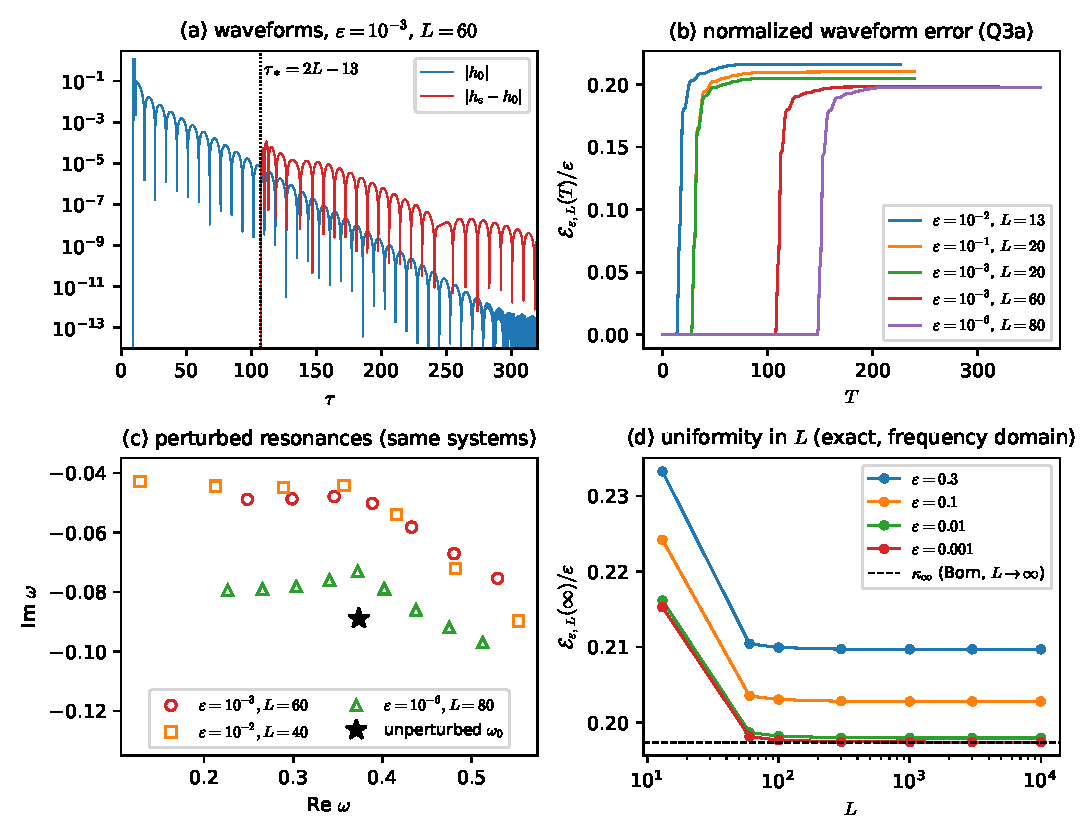
\includegraphics[width=\textwidth]{figs/fig_summary.pdf}
\caption{(a) $\eps=10^{-3}$、$L=60$ 时 $|h_0|$ 与 $|h_\eps-h_0|$（后者在 $\tau<107$ 严格为 0；$\tau\gtrsim280$ 的 $|h_0|$ 为双精度噪声底）；(b) $\cE(T)/\eps$；(c) 同一批系统的扰动共振（最低阻尼 $\Im\omega\approx-0.048$，而 $\Im\omega_0=-0.0890$）；(d) $\cE(\infty)/\eps$ 对 $L$ 直到 $10^4$。}
\label{fig:summary}
\end{figure}

%=====================================================================
\section{设定、记号与精确频域表示}
%=====================================================================
\subsection{基本量}
\begin{itemize}
\item $\rho(x)=2\bigl(1+W_0(e^{x/2-1})\bigr)$（$W_0$ 为 Lambert 函数）；$\rho(0)=2.5569$，$\rho(10)=7.8525$。$V_0>0$ 于全轴，峰值在 $x=2.389$（$\rho=3.2808$），$V_{\max}=0.151287$。$V_\eps=V_0+\eps W_L\ge0$（$\eps>0$），$W_L:=W(\cdot-L)$，$B_L:=[L-1,L+1]$。
\item $C=0.5692357678$；$\|W\|_1=1.2069003$，$\|W\|_2=0.9916556$；$\partial_\tau\psi_0$ 的守恒能量 $E_1=26.12052$。
\item $\|h_0\|^2_{L^2(0,\infty)}=1.006733$（频域 Plancherel）/ $1.006738$（时域两分辨率 Richardson）。其中 97.8\% 来自 prompt 脉冲 $\tau\in[9,11.5]$，1.0\% 来自 $[13,40]$ 的 ringdown，$\tau>40$ 仅 $2\times10^{-5}$。
\item Leaver 连分式：$\omega_0=0.3736716844-0.0889623157i$，$\omega_1=0.3467109969-0.2739148753i$，$\omega_2=0.3010534546-0.4782769832i$；复路径积分得到的 $|\Ain(\omega_{0,1})|<5\times10^{-13}$，零点与 Leaver 值相差 $<10^{-13}$。
\end{itemize}

\subsection{Jost 解与共振}
约定 $e^{-i\omega\tau}$，$\hat f(\omega)=\int_0^\infty e^{i\omega\tau}f\,\dd\tau$（$\Im\omega>0$），$(-\partial_x^2+V-\omega^2)\hat\psi=S_\omega:=-C(W'+i\omega W)$。$\psi_-\sim e^{-i\omega x}$（$x\to-\infty$），$\psi_+\sim e^{i\omega x}$（$x\to+\infty$），$\tilde\psi_+(\omega,\cdot):=\psi_+(-\omega,\cdot)$（实 $\omega$ 时为 $\overline{\psi_+}$）。
\[
\psi_-=\Aout\psi_++\Ain\tilde\psi_+,\qquad \cW_0:=\cW(\psi_-,\psi_+)=2i\omega\Ain,\qquad G_0(\omega;x,y)=-\frac{\psi_-(x_<)\psi_+(x_>)}{\cW_0}.
\]
QNM $\Leftrightarrow$ $\Ain(\omega)=0$。令 $R:=\Aout/\Ain$，$\phi_R:=\psi_-/\Ain$（右入射单位振幅散射态），$I(\omega)=\int\psi_-S_\omega$，$\cA(\omega):=-I/(2i\omega\Ain)$（出射振幅），则 $\hat\psi_0(\omega,x_o)=\cA\,\psi_+(x_o)$，$\hat h=-i\omega\hat\psi(x_o)$。

\subsection[势垒的精确处理与回波公式]{势垒的精确处理与回波公式\enspace\proven}
势垒左侧 $\psi_+^\eps=a\psi_++b\tilde\psi_+$（右侧 $\psi_+^\eps=\psi_+$）。由 $\frac{\dd}{\dd x}\cW(f,g)=\eps W_Lfg$（$f$ 解未扰动方程、$g$ 解扰动方程）得
\begin{gather*}
b=\frac{\eps}{2i\omega}\!\int\! W_L\psi_+\psi_+^\eps,\qquad a=1-\frac{\eps}{2i\omega}\!\int\! W_L\tilde\psi_+\psi_+^\eps,\\
\cW_\eps:=\cW(\psi_-,\psi_+^\eps)=2i\omega(a\Ain-b\Aout)=\cW_0-\eps\!\int\! W_L\psi_-\psi_+^\eps .
\end{gather*}
$\psi_-$ 与源都在势垒左侧，故 $\psi_-$ 不变；代数运算给出（$\beta:=b/a$）
\begin{equation}\label{eq:echo}
\boxed{\;\hat\psi_\eps(\omega,x_o)-\hat\psi_0(\omega,x_o)=\cA(\omega)\,\phi_R(\omega,x_o)\,\frac{\beta(\omega)}{1-\beta(\omega)R(\omega)}=\cA\,\phi_R\,\frac{b}{a-bR}\;}
\end{equation}
即出射波被小势垒以"反射系数" $\beta$ 反射，在两势垒间多次反弹（$\sum_k(\beta R)^{k-1}$），再以 $\phi_R$ 透射到观察者。实 $\omega$ 时通量守恒给出 $|a|^2-|b|^2=1$，故 $|\beta|<1$，$|R|\le1$。\textbf{共振} $\Leftrightarrow$ $F(\omega):=\Ain(\omega)-\beta(\omega)\Aout(\omega)=0$。Born 项：$\hat h_1=-i\omega\cA\phi_R\,b_1$，$b_1=\frac{1}{2i\omega}\int W_L\psi_+^2$；大 $L$ 时 $\psi_+=e^{i\omega x}(1+\frac{3i}{\omega\rho}+O(\rho^{-2}))$，$b_1\approx e^{2i\omega L}\hat W(-2\omega)/(2i\omega)$。（频域 $\hat h_0,\hat h_1$ 与时域波形的数值 Laplace 变换在 $\omega=0.05\ldots3$ 相对吻合到 $\lesssim10^{-5}$。）

\subsection[源--势垒--探测器形式]{源--势垒--探测器形式\enspace\proven}
令 $K_L(\omega)=W_L^{1/2}R_0(\omega)W_L^{1/2}$（势垒$\to$势垒），$D_L(\omega)=W_L^{1/2}G_0(\omega;\cdot,x_o)$（势垒$\to$探测器），$S_L(\omega)=W_L^{1/2}R_0(\omega)S_\omega=W_L^{1/2}\hat\psi_0$（源$\to$势垒）。由 $R_\eps=R_0-\eps R_0W_LR_\eps$：
\begin{equation}\label{eq:BS}
\boxed{\;\delta\hat\psi(\omega,x_o)=-\eps\,\big\langle D_L(\omega),\,(1+\eps K_L(\omega))^{-1}S_L(\omega)\big\rangle\;}\qquad(\text{双线性配对}).
\end{equation}
它在闭上半平面成立，并亚纯延拓到下半平面，\textbf{其极点正是共振（$1+\eps K_L$ 不可逆处）}。

\subsection[\texorpdfstring{Plancherel 与 $\sup_T$}{Plancherel 与 sup over T}]{Plancherel 与 $\sup_T$\enspace\proven}
$\cE(T)$ 对 $T$ 单调不减，故 $\sup_T\cE(T)=\cE(\infty)$，且（$h$ 为实信号）
\[
\cE(\infty)^2=\frac{1}{\pi\|h_0\|^2}\int_0^\infty|\hat h_\eps(\omega)-\hat h_0(\omega)|^2\,\dd\omega .
\]
严格化：$\psi$ 至多多项式增长（能量守恒 + 有限传播速度），在 $\Im\omega=\eta>0$ 上用 Plancherel，再令 $\eta\downarrow0$（单调收敛）。

%=====================================================================
\section{A 部分：因果传播与首阶波形}
%=====================================================================
\begin{theorem}[因果]\label{thm:causal}\proven\enspace 对任意 $L>12$ 与任意 $\eps$：(i) $h_\eps\equiv h_0\equiv0$ 于 $[0,9]$；(ii) $h_\eps(\tau)=h_0(\tau)$ 对一切 $0\le\tau\le2L-13$。
\end{theorem}
\begin{proof}
$\Box+V$（$V$ 有界光滑）有单位传播速度（截断光锥上的能量估计）。$\supp\psi_0(\tau,\cdot)\subset[-1-\tau,1+\tau]$，$x_o=10$ 在 $\tau<9$ 时不在其中，得 (i)。$u:=\psi_\eps-\psi_0$ 满足 $(\Box+V_\eps)u=F:=-\eps W_L\psi_0$，零初值；$\supp F\subset\{(s,y):y\in B_L,\ y\le1+s\}$。若 $u(\tau,x_o)\ne0$，须有 $(s,y)\in\supp F$ 使 $\tau-s\ge y-x_o$，从而 $\tau\ge s+y-10\ge(y-1)+y-10\ge2(L-1)-11=2L-13$。故 $u(\cdot,x_o)\equiv0$ 于 $[0,2L-13]$，其 $\tau$-导数 $h_\eps-h_0$ 亦然。
\end{proof}

\begin{proposition}[最优性与平坦性]\label{prop:sharp}\sketch\enspace 对任意 $\eps>0$ 与 $\delta>0$，$h_\eps-h_0\not\equiv0$ 于 $(\tauS,\tauS+\delta)$（$\tauS=2L-13$），但其所有导数在 $\tauS$ 处为 0。
\end{proposition}
\noindent\textbf{概要.} 1+1 维 $\Box+V$ 的推迟基本解为 $\tfrac12\theta(t-s-|x-y|)\,\cR(t,x;s,y)$，Riemann 函数 $\cR$ 连续且在光锥边界上 $\equiv1$。对 $\psi_0$ 用同一表示：在右波前 $y-s\uparrow1$ 附近 $\psi_0=CW(y-s)(1+O(\eta^2))$，因为势修正正比于 $\int_{1-\eta}^1W\ll W(1-\eta)$（$W$ 在端点无穷阶平坦）。于是在角点 $(s,y)=(L-2,L-1)$ 附近 $W_L\psi_0>0$，而 $u(\tauS+\delta,x_o)=-\frac{\eps}{2}\iint_{D_\delta}\cR_\eps W_L\psi_0<0$（$D_\delta$ 为非空开集，$\cR_\eps=1+O(\delta)$）。若 $\dot u(\cdot,x_o)\equiv0$ 于该区间，$u$ 将恒为 $u(\tauS)=0$，矛盾。平坦性来自 $W$ 与 $\psi_0$ 波前的无穷阶平坦；对 Born 项 $u_1$ 同理，故 $h_1\not\equiv0$ 于 $(\tauS,\tauS+\delta)$。

\numer\enspace 在 Courant 数 1 的 GPP 菱形格式中（数值光锥与物理光锥精确一致），$u(\cdot,x_o)$ 在 $\tau<2L-13+2h$ 上\textbf{按位严格为 0}；9 组 $(\eps,L)$ 在 $h=1/128,1/256$ 下均如此（起始 $=2L-13+2h\to2L-13$）。紧随其后的值极小（$L=60,\eps=10^{-3}$：$\cE(\tauS+1)=3.5\times10^{-6}$，$\cE(\tauS+2)=3.8\times10^{-5}$），与无穷阶平坦一致。

\subsection{Duhamel/Born 展开与余项}
$u=\eps u_1+\eps^2u_2$，$u_1=-\cG_0[W_L\psi_0]$，$u_2=-\cG_\eps[W_Lu_1]$（$\cG_V$ 为推迟解算子）：
\[
h_\eps-h_0=\eps h_1+\eps^2r_\eps,\qquad h_1(\tau)=-\partial_\tau\!\int_0^\tau\!\!\int G_0^{\rm ret}(\tau-s;x_o,y)\,W(y-L)\,\psi_0(s,y)\,\dd y\,\dd s,
\]
频域 $\hat h_1=i\omega\,\psi_-(x_o)I\,\cW_0^{-2}\int W_L\psi_+^2$。余项控制（三种互补的范围）：
\begin{itemize}
\item \textbf{(R1)}\,\proven\enspace 全部 $\eps>0$、$L>12$、$T$（初等能量法，同定理~\ref{thm:A} 的证明）：
$\|h_\eps-h_0-\eps h_1\|_{L^2(0,T)}\le0.2641\,\eps^2[\sigma_T^7-\sigma_*^7]_+^{1/2}$，$\sigma_T=T+2-L$，$\sigma_*=L-11$（常数 $=\|W\|_2^2E_1^{1/4}\sqrt{8/567}$）。
\item \textbf{(R2)}\,\condJ\enspace 对所有 $T$ 一致：若 $\eps K_3(L)<1$，则
\[\|h_\eps-h_0-\eps h_1\|_{L^2(0,\infty)}\le\frac{\eps^2K_2K_3(L)N_L}{1-\eps K_3(L)}.\]
\item \textbf{(R3)}\,\numer\enspace $(\cE(\infty)/\eps-\|h_1\|/\|h_0\|)/\eps\approx0.054$--$0.10$（表~\ref{tab:largeL}），远小于 (R2) 的 $O(\eps L)$ 悲观估计。
\end{itemize}

\subsection{(Q3a)(Q3b) 的阶数：generic、特殊抵消、归一化失效}
\begin{table}[h]
\centering\small
\begin{tabularx}{\textwidth}{@{}l>{\raggedright\arraybackslash}X>{\raggedright\arraybackslash}X@{}}
\toprule
时间范围 & $\cE(T)$ & $\cM(T)$\\\midrule
$T\le9$ & 0（精确） & \textbf{归一化失效}：$\|h_0\|_T=\|h_\eps\|_T=0$，无定义\\
$9<T\le2L-13$ & 0（精确，所有阶） & 0（精确，所有阶）\\
$T>2L-13$ & \textbf{generic 一阶}：$\eps c_1(T)+O(\eps^2)$，$c_1=\|h_1\|_T/\|h_0\|>0$，在 $\tauS$ 处无穷阶平坦 & \textbf{特殊抵消}：一阶项恒为 0（只依赖夹角，平行分量不贡献）；$\cM=\eps^2m_2+O(\eps^3)$，$m_2=\|P_\perp h_1\|_T^2/(2\|h_0\|_T^2)>0$\\\bottomrule
\end{tabularx}
\end{table}
\proven\enspace $m_2>0$：若 $h_1=\lambda h_0$ 于 $[0,T]$，因 $h_1\equiv0$ 于 $[0,\tauS]$ 而 $h_0\not\equiv0$ 于 $(9,\tauS)$，得 $\lambda=0$，与命题~\ref{prop:sharp} 矛盾。\proven\enspace 实信号的精确界：$\cM(T)=1-|\cos\theta|\le\sin^2\theta\le\|h_\eps-h_0\|_T^2/\|h_0\|_T^2=\cE(T)^2\|h_0\|_\infty^2/\|h_0\|_T^2$。\textbf{(Q3a) 用 $h_0$ 的总能量归一化}，prompt 脉冲占 97.8\%，所以 $\tau\approx2L$ 处"回波/已衰减背景"的巨大比值不进入 $\cE$（\S\ref{sec:td}）。

\begin{table}[h]
\centering\small
\caption{时域结果（GPP，$h=1/256$；括号内为 Born 预测 $m_2$）。$\eps=10^{-6}$ 时 $\cM\sim10^{-14}$ 接近双精度舍入。}\label{tab:td}
\begin{tabular}{@{}cccccc@{}}
\toprule
$\eps$ & $L$ & $\cE(\infty)/\eps$ & $\cE(\tauS+5)$ & $\cM(T_{\max})/\eps^2$ & ($m_2$)\\\midrule
$10^{-1}$ & 20 & 0.210139 & $1.39\times10^{-2}$ & 0.02207 & (0.02096)\\
$10^{-2}$ & 20 & 0.205375 & $1.36\times10^{-3}$ & 0.02109 & (0.02096)\\
$10^{-3}$ & 20 & 0.204818 & $1.36\times10^{-4}$ & 0.02098 & (0.02096)\\
$10^{-2}$ & 13 & 0.216145 & $1.39\times10^{-3}$ & 0.02336 & (0.02315)\\
$10^{-3}$ & 30 & 0.200582 & $1.33\times10^{-4}$ & 0.02012 & (0.02011)\\
$10^{-2}$ & 40 & 0.199687 & $1.32\times10^{-3}$ & 0.01994 & (0.01982)\\
$10^{-4}$ & 50 & 0.198442 & $1.31\times10^{-5}$ & 0.01969 & (0.01969)\\
$10^{-3}$ & 60 & 0.198155 & $1.30\times10^{-4}$ & 0.01964 & (0.01962)\\
$10^{-6}$ & 80 & 0.197765 & $1.30\times10^{-7}$ & 0.01965 & (0.01956)\\\bottomrule
\end{tabular}
\end{table}

%=====================================================================
\section{B 部分：同一系统的极点迁移}
%=====================================================================
\subsection[一阶位移]{一阶位移\enspace\proven（一阶微扰）\enspace\numer}
在简单根 $\omega_0$ 处，$F(\omega_0+\delta)=\Ain'\delta-\beta\Aout+\dots$，得
\[
\delta\omega^{(1)}=\eps\frac{b_1(\omega_0)\Aout(\omega_0)}{\Ain'(\omega_0)}=\frac{\eps\int W_L\psi_-\psi_+}{\partial_\omega\cW_0(\omega_0)}=:\eps\kappa(L),\qquad
\kappa(L)\simeq\frac{\Aout\hat W(-2\omega_0)}{2i\omega_0\Ain'}\,e^{2i\omega_0L}\,(1+O(L^{-1})).
\]
数值：$\Aout(\omega_0)=-1.029204+0.057780i$，$\Ain'(\omega_0)=-10.438806-0.197380i$，$\hat W(-2\omega_0)=1.157180+0.024636i$，$|\kappa_\infty|=0.14875$。
\begin{table}[h]
\centering\small
\begin{tabular}{@{}lcccccc@{}}
\toprule
$L$ & 13 & 20 & 30 & 40 & 60 & 100\\\midrule
$|\kappa(L)|$ & 1.241 & 4.480 & 27.64 & 167.9 & 6061 & $7.651\times10^6$\\
$|\kappa|e^{-2\gamma_0L}$ & 0.1228 & 0.1276 & 0.1329 & 0.1362 & 0.1400 & 0.1434 $\to$ 0.1488\\\bottomrule
\end{tabular}
\end{table}

\noindent 第一泛音：$|\kappa_1|e^{-2\gamma_1L}$ 从 0.127（$L=13$）增至 0.249（$L=100$），$\gamma_1=0.2739$。\textbf{适用条件}：$\Lambda\ll1$ 且 $|\delta\omega^{(1)}|\ll$ 与其它根的距离。

\subsection[\texorpdfstring{真正的展开参数与 Lambert-$W$ 重求和}{真正的展开参数与 Lambert-W 重求和}]{真正的展开参数与 Lambert-$W$ 重求和\enspace\sketch\enspace\numer}
在 $\omega_0$ 的固定小圆盘内写 $\beta=\eps e^{2i\omega L}B(\omega;\eps,L)$，$B$ 对 $L\ge L_0,\eps\le\eps_0$ 一致有界解析。零点满足
\[
\delta=\delta^{(1)}e^{2iL\delta}\bigl(1+O(\delta)\bigr)\ \Longrightarrow\ \delta_k=\frac{i}{2L}W_k\bigl(-2iL\,\delta^{(1)}\bigr)\bigl(1+O(\delta)\bigr).
\]
$k=0$ 分支连续接到 $\omega_0$；在模型方程中，它的 $\eps$ 幂级数即 $W_0(z)$ 的 Taylor 级数，\textbf{收敛当且仅当 $\Lambda:=2L|\delta\omega^{(1)}|<1/e$}（$z=-1/e$ 处 $W_0$ 与 $W_{-1}$ 碰撞，即主模与一个空腔模的例外点）。故控制展开的是 $\Lambda\approx0.30\,L\eps e^{2\gamma_0L}$：大 $L$ 时即使 $|\delta\omega^{(1)}|\ll1$，线性化也可能已失效。$k\ne0$ 为两势垒间的空腔模，间距 $\approx\pi/L$。

\begin{table}[h]
\centering\footnotesize\setlength{\tabcolsep}{4pt}
\caption{一阶公式、Lambert-$W$（$k=0$）与精确根（复 Jost 函数 + Muller 迭代，$|F|/|\Aout|<10^{-9}$）。}\label{tab:lw}
\begin{tabular}{@{}cccccccc@{}}
\toprule
$\eps$ & $L$ & $\Lambda$ & 一阶 $\omega_0+\delta^{(1)}$ & Lambert-$W$ & 精确根 & 一阶误差 & LW 误差\\\midrule
$10^{-3}$ & 20 & 0.179 & $0.37207-0.08478i$ & $0.37246-0.08529i$ & $0.37260-0.08525i$ & $7.1\times10^{-4}$ & $1.4\times10^{-4}$\\
$10^{-6}$ & 60 & 0.727 & $0.37955-0.09045i$ & $0.37842-0.08738i$ & $0.37825-0.08750i$ & $3.2\times10^{-3}$ & $2.1\times10^{-4}$\\
$10^{-5}$ & 50 & 1.01 & $0.37563-0.09888i$ & $0.38583-0.09093i$ & $0.38473-0.09112i$ & $1.2\times10^{-2}$ & $1.1\times10^{-3}$\\
$10^{-3}$ & 30 & 1.66 & $0.34775-0.07935i$ & $0.36473-0.07789i$ & $0.36580-0.07721i$ & $1.8\times10^{-2}$ & $1.3\times10^{-3}$\\
$10^{-6}$ & 70 & 5.07 & $0.39622-0.06062i$ & $0.37643-0.07960i$ & $0.37672-0.07996i$ & $2.8\times10^{-2}$ & $4.7\times10^{-4}$\\
$10^{-4}$ & 50 & 10.1 & $0.39323-0.18819i$ & $0.39362-0.07477i$ & $0.39334-0.07690i$ & $1.1\times10^{-1}$ & $2.1\times10^{-3}$\\
$10^{-8}$ & 100 & 15.3 & $0.34966-0.16160i$ & $0.36378-0.08018i$ & $0.36429-0.07986i$ & $8.3\times10^{-2}$ & $6.0\times10^{-4}$\\
$10^{-6}$ & 80 & 34.6 & $0.27280\,\bm{+0.10198i}$ & $0.37148-0.07281i$ & $0.37228-0.07307i$ & $2.0\times10^{-1}$ & $8.5\times10^{-4}$\\\bottomrule
\end{tabular}
\end{table}

\begin{figure}[h]
\centering
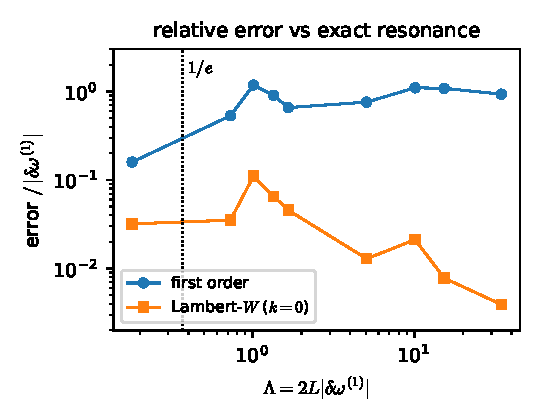
\includegraphics[width=0.52\textwidth]{figs/fig_lambertw.pdf}
\caption{相对误差（除以 $|\delta\omega^{(1)}|$）对 $\Lambda$：一阶公式在 $\Lambda\gtrsim1$ 已完全失效，Lambert-$W$ 主分支保持 $10^{-3}$--$10^{-1}$ 的相对精度。}\label{fig:lw}
\end{figure}

表~\ref{tab:lw} 最后一行：线性外推甚至给出错误的"增长模"（$\Im>0$），而重求和与精确根一致。空腔分支（$\eps=10^{-6},L=80$，$k=-4\ldots4$）：精确根 $\Re\omega=0.227\ldots0.513$，相邻间距 0.030--0.039（$\pi/80=0.0393$），$\Im\omega\in[-0.097,-0.073]$；Lambert-$W$ 对 $k\ne0$ 的误差 $\le0.012$。

\subsection[\texorpdfstring{双重极限 $L=c\log(1/\eps)$}{双重极限 L = c log(1/ε)}]{双重极限 $L=c\log(1/\eps)$\enspace\condJa\enspace\numer}
\begin{proposition}\label{prop:double}设 $L=c\log(1/\eps)$，$\eps\to0$。
(a) 若 $\gamma_n<1/(2c)$，恰有一个共振收敛到 $\omega_n$，且 $|\omega-\omega_n|\sim|\kappa_{\infty,n}|\eps^{1-2\gamma_nc}\to0$；
(b) 若 $\gamma_n>1/(2c)$ 且 $B_\infty\Aout(\omega_n)\ne0$（$n=0$：$\Aout(\omega_0)=-1.029+0.058i$，$\hat W(-2\omega_0)=1.157+0.025i$），没有共振收敛到 $\omega_n$；在紧集 $K\subset\{\Im\omega>-1/(2c)\}$ 内共振只收敛到 $\gamma_n<1/(2c)$ 的 $\omega_n$，而共振以密度 $L/\pi$ 聚集到直线 $\Im\omega=-1/(2c)$（\textbf{新分支}），$\Im\omega_k=-\frac{1}{2L}\log\frac{1}{\eps|BR|}+o(L^{-1})$；
(c) 在 $\{\Im\omega<-1/(2c)\}$ 的紧集内，共振收敛到 $B_\infty\Aout$ 的零点（$B_\infty=\hat W(-2\omega)/(2i\omega)$）。
\end{proposition}
\begin{proof}
在 $K$ 上 $|\eps e^{2i\omega L}|=\eps^{1+2c\Im\omega}$。上方区域 $\beta\Aout\to0$ 一致成立，对 $F$ 用 Hurwitz 定理；下方区域 $\Ain/(\eps e^{2i\omega L})\to0$，对 $F/(\eps e^{2i\omega L})$ 用 Hurwitz 定理。所需输入 (J-asym)：$B(\omega;\eps,L)\to B_\infty$ 在紧集上一致成立，由 $\psi_\pm$ 的一致渐近展开给出（本文数值使用并核验了该展开）。(a) 的速率来自重求和分析。（(c) 未做数值检验。）
\end{proof}
\textbf{阈值}：基模 $c_*=1/(2\gamma_0)=5.6203$；第一泛音 $c_{1*}=1/(2\gamma_1)=1.8254$。$c=c_*$ 时 $\Lambda\sim2L|\kappa_\infty|\to\infty$ 缓慢增长，位移以 $O(\log L/L)$ 趋零。

\begin{table}[h]
\centering
\caption{沿 $k=0$ 分支追踪的精确根。}\label{tab:double}
\resizebox{\textwidth}{!}{%
\begin{tabular}{@{}cccccccl@{}}
\toprule
$c$ & $\eps=10^{-2}$ & $10^{-3}$ & $10^{-4}$ & $10^{-6}$ & $10^{-8}$ & $10^{-10}$ & 预测极限\\\midrule
3 & $0.35291-0.09673i$ & $0.37075-0.08552i$ & $0.37441-0.08750i$ & $0.37371-0.08918i$ & $0.37365-0.08895i$ & $0.37367-0.08896i$ & $\omega_0$，速率 $\eps^{0.466}$\\
4 & $0.38254-0.07424i$ & $0.37736-0.07967i$ & $0.37424-0.08304i$ & $0.37216-0.08737i$ & $0.37299-0.08925i$ & $0.37369-0.08916i$ & $\omega_0$，速率 $\eps^{0.288}$\\
5 & $0.34599-0.06716i$ & $0.38840-0.07548i$ & $0.37205-0.07540i$ & $0.37932-0.08124i$ & $0.38322-0.08617i$ & $0.37039-0.08528i$ & $\omega_0$，极慢 $\eps^{0.110}$\\
6.5 & $0.36499-0.05505i$ & $0.37929-0.06129i$ & $0.38702-0.06534i$ & $0.36813-0.06695i$ & $0.37884-0.06937i$ & $0.36810-0.07033i$ & $\Im\to-0.0769$\\
8 & $0.37876-0.04886i$ & $0.36977-0.05169i$ & $0.36424-0.05371i$ & $0.38243-0.05699i$ & $0.37328-0.05779i$ & $0.36747-0.05853i$ & $\Im\to-0.0625$\\\bottomrule
\end{tabular}}
\end{table}

\begin{figure}[h]
\centering
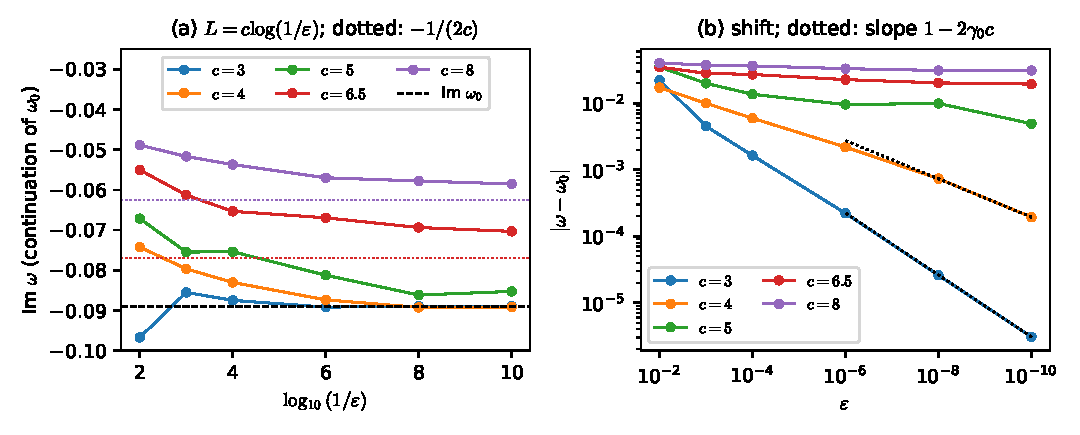
\includegraphics[width=\textwidth]{figs/fig_double_limit.pdf}
\caption{双重极限。(a) $\omega_0$ 延续根的虚部：$c<c_*$ 回到 $\Im\omega_0$，$c>c_*$ 趋向点线 $-1/(2c)$；(b) $|\omega-\omega_0|$，黑色点线为预测斜率 $1-2\gamma_0c$。}\label{fig:double}
\end{figure}

$c=3$ 时 $|\omega-\omega_0|$ 从 $\eps=10^{-6}$ 到 $10^{-10}$ 缩小 72 倍（指数 0.46，预测 0.466）。$c=8$ 时向 $-1/(2c)$ 的收敛带 $O(\log L/L)$ 修正：Lambert 渐近 $\Im\delta\approx(\log\Lambda-\log\log\Lambda)/(2L)$ 给出 $\eps=10^{-10}$ 时 $-0.0588$，精确值 $-0.0585$。

\subsection[\texorpdfstring{与同一 $(\eps,L)$ 时域信号的比较}{与同一 (ε,L) 时域信号的比较}]{与同一 $(\eps,L)$ 时域信号的比较\enspace\proven+\numer}\label{sec:td}
取 $(\eps,L)=(10^{-3},60)$（$c=8.69>c_*$，$\Lambda=727$）。最低阻尼共振为 $0.34592-0.04795i$、$0.29867-0.04873i$、$0.38873-0.05023i$、\ldots（图~\ref{fig:summary}(c)），阻尼比 $\gamma_0$ 小约 46\%。\textbf{辐角原理}（圆周 240 点，最大相位步长 0.19 rad）确认 $|\omega-\omega_0|<0.035$ 内共振数为 0（$\eps=10^{-6},L=80$ 时半径 0.012 内也为 0）。然而：
\begin{itemize}
\item \textbf{因果}：$h_\eps\equiv h_0$ 于 $[0,107]$。在窗口 $[82,106]$ 对 $h_\eps$ 做单模自由拟合，得 $\bm{0.373672-0.088962i}$（相对残差 $7\times10^{-7}$），即\textbf{未扰动的} $\omega_0$；$\eps=10^{-4},L=50$ 时同样得到 $0.373675-0.088962i$。
\item \textbf{pole residues}：$\operatorname{Res}_{\omega_0}\hat h_0=0.046927+0.014382i$，预测时域振幅 $-i\operatorname{Res}=0.014382-0.046927i$（$h_0\supset2\Re[-i\operatorname{Res}\,e^{-i\omega_0\tau}]$）；在 $[25,70]$ 上用 $\omega_0,\omega_1$ 最小二乘得 $0.014342-0.046922i$（相对偏差 $3\times10^{-3}$）。
\item \textbf{回波}：$\tau>107$ 时 $\delta h$ 为 prompt 脉冲的 $O(\eps)$ 反射（峰值 $\approx0.12\eps$）加其 ringdown。由 \eqref{eq:echo}，$\cA\phi_R\beta\propto\Ain^{-2}$，即在\textbf{未扰动} $\omega_n$ 处为二阶极点。数值：在 $[\tauS+30,\tauS+80]$ 用 $\omega_0,\omega_1$ 且带 $\tau e^{-i\omega\tau}$ 久期项拟合，相对残差 $3\times10^{-4}$；单个简单极点 $\omega_0$ 残差 47\%（四组 $(\eps,L)$ 结果相同）。\textbf{扰动后的新谱不直接出现在任何有限时间窗中。}
\item \textbf{相对误差 vs 能量归一化误差}：回波窗口 $(\tauS,\tauS+25)$ 内 $\max|\delta h|/\max|h_0|=17.5$（$\eps e^{2\gamma_0L}=43$），而 $\cE(\infty)=1.98\times10^{-4}$，$\cM(\infty)=1.96\times10^{-8}$。九组数据中该比值 $=(0.16\text{--}0.59)\,\eps e^{2\gamma_0L}$：\textbf{控制极点位移的参数恰好控制回波时刻的相对误差，而不是 (Q3a)。}
\item \textbf{新共振的 residue 与适用时间窗}\,\exactlow：空腔零点 $\omega_k$ 处 $\frac{\beta}{1-\beta R}$ 的留数 $\approx\frac{i}{2LR(\omega_k)}$，每个新模激发系数为 $O(1/L)$，\textbf{不随 $\eps$ 变小}；但它们只在 $\tau\gtrsim2L$ 起效，此时 $|e^{-i\omega_k\tau}|\approx\eps$，约 $L$ 个模叠加出 $O(\eps)$ 回波。因此在 $\tau<2L-13$ 上，有限个扰动 QNM 之和不能代表 $h_\eps$。正确的时间窗表述是回波展开 $\delta\hat\psi=\cA\phi_R\sum_{k\ge1}\beta^kR^{k-1}$：第 $k$ 项幅度 $O(\eps^k)$，到达时间约 $2kL$；在 $[0,2(k+1)L-13)$ 内只有前 $k$ 项起作用，每一项的 ringdown 由\textbf{未扰动} $\omega_n$ 的 $(k+1)$ 阶极点给出。
\item \textbf{prompt response}：$\|h_0\|^2$ 的 97.8\% 来自 prompt 脉冲，它经小势垒反射后成为回波主体。回波谱权重集中于 $\omega\in[0.3,1.9]$（90\% 分位 1.32，99\% 分位 1.87）。
\item \textbf{branch cut / tail}：未扰动尾巴 $h_0\sim\tau^{-8}$ 对 $\|h_0\|^2$ 贡献可忽略；双精度时域无法分辨（$\tau\gtrsim280$ 噪声底 $\sim10^{-13}$；在 $\tau\in[800,1600]$ 测尾巴比值的尝试被舍入噪声淹没，\textbf{不作数值声称}）。\exactlow\enspace 穿过势垒的静态正则解 $u_0=\rho^3/8$ 在势垒外侧的 $\rho^3$ 系数变为 $A=\tfrac18+\eps\int W_Lu_0v_0\approx\tfrac18(1+\eps\|W\|_1\rho_L/5)$，由此\conj\enspace 晚期尾巴振幅按 $(8A)^{-2}$ 缩放（$L=20,\eps=0.1$ 时 $8A=1.444$），但对 $\cE$ 的贡献 $\lesssim\eps^2L^2\int_{2L}^\infty\tau^{-16}$。低频处 Jost 基下 $|\beta|\to1$（$\omega\sim10^{-3}$ 时 $|\beta|>1-10^{-9}$），空腔增强 $|1/(1-\beta R)|$ 可达 $10^5$，但这些频率对 $\cE^2$ 的贡献 $\le2\times10^{-9}$。
\end{itemize}

%=====================================================================
\section{C 部分：统一观测稳定性}
%=====================================================================
\subsection{初等能量界}
\begin{theorem}[全参数]\label{thm:A}\proven\enspace 对一切 $\eps>0$、$L>12$、$T\ge0$：
\[
\cE_{\eps,L}(T)\le K_A\,\eps\,\bigl[(T+2-L)^4-(L-11)^4\bigr]_+^{1/2},\qquad K_A=\tfrac{\sqrt2}{3}\|W\|_2E_1^{1/4}/\|h_0\|=1.0533 .
\]
\end{theorem}
\begin{proof}
(i) $V_\eps\ge0$，故 $(\Box+V)\phi=F$ 零初值时 $\sqrt{E_V[\phi](\tau)}\le2^{-1/2}\int_0^\tau\|F(s)\|_{L^2}\dd s$。
(ii) $\psi_0(s,\cdot)$ 支在 $x\le1+s$，于是对 $x\ge L-1$：$|\psi_0(s,x)|\le\sqrt{1+s-x}\,\|\partial_x\psi_0\|\le\sqrt{2\sigma_s}$（$\sigma_s=s+2-L$，$E_{V_0}[\psi_0]=1$）；$\partial_\tau\psi_0$ 同理，把 1 换成 $E_1$。
(iii) $u=\psi_\eps-\psi_0$ 与 $\dot u$ 均为零初值（$\ddot u(0)=-\eps W_L\psi_0(0)=0$），源分别为 $-\eps W_L\psi_0$、$-\eps W_L\dot\psi_0$，故 $\sqrt{E[u]}\le\frac23\eps\|W\|_2\sigma^{3/2}$，$\sqrt{E[\dot u]}\le\frac23\eps\|W\|_2E_1^{1/2}\sigma^{3/2}$。
(iv) 一维迹不等式 $|g(x_o)|^2\le\|g\|\|g'\|$ 给出 $|\dot u(\tau,x_o)|^2\le2\sqrt{E[u]E[\dot u]}\le\frac89\eps^2\|W\|_2^2E_1^{1/2}\sigma^3$。
(v) 对 $\tau$ 从 $\tauS$（$\sigma=L-11$）积分到 $T$。同样论证用于 $u_2$ 给出 (R1)。
\end{proof}
\begin{corollary}[对数窗口]若 $T\le\kappa L$、$L=c\log(1/\eps)$，则 $\cE\le K_A(\kappa-1)^2c^2\eps\log^2(1/\eps)(1+o(1))$，即对任意 $\alpha<1$ 有 $\cE\le C_\alpha\eps^\alpha$。
\end{corollary}
\textbf{限制来源}：纯粹来自\textbf{估计工具}（未用任何色散或局部衰减）。界相当粗（$L=20$、$T=\tauS+20$ 时给出 $881\eps$，实际约 $0.2\eps$），但严格、无条件，且与极点位移大小无关。

\subsection{源--探测器 resolvent 界}
定义（sup 取闭上半平面；由 J2 等于实轴上的 sup）
\[
K_2=\sup_{L\ge L_0}\sup_{\Im\omega\ge0}\|\omega D_L(\omega)\|_{L^2},\quad
K_3(L)=\sup_{\Im\omega\ge0}\|K_L(\omega)\|_{L^2\to L^2},\quad
N_L=\|W_L^{1/2}\psi_0\|_{L^2(\mathbb R_+\times\mathbb R)} .
\]
\begin{theorem}\label{thm:B}\condJ\enspace 若 $\eps K_3(L)<1$，则
\[
\sup_{T\ge0}\cE_{\eps,L}(T)\le\frac{\eps K_2N_L}{(1-\eps K_3(L))\|h_0\|},\qquad
\|h_\eps-h_0-\eps h_1\|_{L^2(0,\infty)}\le\frac{\eps^2K_2K_3(L)N_L}{1-\eps K_3(L)} .
\]
\end{theorem}
\begin{proof}
对 $\Im\omega=\eta>0$，由 \eqref{eq:BS}：$|\omega\,\delta\hat\psi(\omega,x_o)|\le\eps\|\omega D_L\|\,\|(1+\eps K_L)^{-1}\|\,\|S_L\|\le\frac{\eps K_2}{1-\eps K_3}\|W_L^{1/2}\hat\psi_0(\omega)\|$。对 $\Re\omega$ 平方积分并用 Plancherel：$\int e^{-2\eta\tau}|\dot u(\tau,x_o)|^2\le(\frac{\eps K_2}{1-\eps K_3})^2\iint e^{-2\eta\tau}W_L|\psi_0|^2\le(\cdots)^2N_L^2$，再令 $\eta\downarrow0$。第二式把 Neumann 级数多展一项。
\end{proof}
\begin{assumption}[条件 J]标准 RW 散射论事实，本文未重新证明。(J1) $\omega\mapsto\omega D_L(\omega)$（$L^2$ 值）与 $K_L(\omega)$（算子值）在闭上半平面（含 $\omega=0$）连续有界，并在 $|\omega|\to\infty$ 时衰减；$N_L<\infty$。(J2) 由 (J1)、次调和性与 Phragmén--Lindelöf，上半平面的 sup 等于实轴上的 sup。对 $s=0$ 的 RW 势低能分析见 \cite{DSS}；$s=2$ 的对应结论未逐条核对文献，故列为假设。
\end{assumption}

\begin{table}[h]
\centering
\caption{实轴上的常数\ \numer（$\omega$ 网格：$10^{-4}$--$0.05$ 取 150 个对数点，$0.05$--$12$ 步长 0.002；势垒上 64 点 Gauss--Legendre；$\psi_-$ 从视界侧直接积分以避免低频相消）。}\label{tab:K}
\resizebox{\textwidth}{!}{%
\begin{tabular}{@{}cccccccccc@{}}
\toprule
$L$ & $\rho(L)$ & $K_2(L)$（取于 $\omega$） & $K_3(L)$（取于 $\omega$） & $\|K_L(0)\|$ [静态 $\|W\|_1(\frac{\rho}{5}+\frac13)$] & $N_L$ & 界 $K_2N_L/\|h_0\|$ & 实际 $\cE(\infty)/\eps$ & $1/(2K_3)$ & $\sup_{\omega\ge0.1}\omega\|K_L\|$\\\midrule
13 & 10.18 & 1.364 (0.328) & 5.79 (0.256) & 2.69 [2.86] & 0.5778 & 0.786 & 0.2152 & 0.086 & 1.58\\
15 & 11.82 & 1.328 (0.330) & 6.41 (0.228) & 3.07 [3.26] & 0.5760 & 0.763 & 0.2107 & 0.078 & 1.57\\
20 & 16.09 & 1.281 (0.332) & 8.14 (0.174) & 4.07 [4.29] & 0.5734 & 0.732 & 0.2048 & 0.061 & 1.54\\
30 & 25.11 & 1.248 (0.332) & 11.95 (0.116) & 6.23 [6.46] & 0.5715 & 0.711 & 0.2005 & 0.042 & 1.52\\
40 & 34.43 & 1.237 (0.332) & 15.95 (0.086) & 8.46 [8.71] & 0.5708 & 0.704 & 0.1991 & 0.031 & 1.52\\
60 & 53.50 & 1.230 (0.332) & 24.19 (0.056) & 13.06 [13.32] & 0.5704 & 0.699 & 0.1981 & 0.021 & 1.28\\
100 & 92.38 & 1.226 (0.332) & 41.02 (0.033) & 22.44 [22.70] & 0.5702 & 0.697 & 0.1976 & 0.012 & 1.24\\
200 & 190.90 & 1.225 (0.332) & 83.72 (0.016) & 46.21 [46.48] & 0.5701 & 0.696 & -- & 0.006 & 1.21\\\bottomrule
\end{tabular}}
\end{table}

$K_2=\sup_LK_2(L)=1.364$（$L=13$），$\sup_LN_L=0.578$；$K_3(L)/L\approx0.40$--$0.45$，最大值位于 $\omega\approx3.3/L$（近区与远区交界）。定理~\ref{thm:B} 的界比实际值大约 3.6 倍。

\begin{corollary}\condJ\enspace 由于 $K_3(L)\approx0.41L$，只要 $\eps K_3(L)\le\frac12$（约 $\eps L\lesssim1.1$--$1.2$），就有 $\sup_T\cE\le2\eps K_2\sup_LN_L/\|h_0\|=1.571\,\eps$，与 $T,L$ 无关。\textbf{这覆盖了所有 $L=c\log(1/\eps)$、任意 $c>0$（$\eps$ 足够小）}，包括 $c>c_*$ 这类极点已 $O(1)$ 迁移的情形。因此在 (Q3c) 要求的对数窗口内，统一命题以 $\alpha=1$、无对数修正成立。
\end{corollary}
\textbf{限制来源}：$K_3(L)=O(L)$ 来自\textbf{低频}：远区 $\|K_L(\omega)\|\approx\|W\|_1/(2\omega)$，增长到 $\omega\approx3.3/L$ 才饱和；近区静态 Green 函数 $G_0(0;y,y)=\rho/5+1/3+O(\rho^{-1})$（\exactlow）同样线性增长。这是\textbf{低频 + 估计工具}的限制：最坏频率上的范数被当成了所有频率的放大因子；而回波能量集中的 $\omega\in[0.3,1.9]$ 上 $\omega\|K_L\|\le1.6$。它\textbf{不是}共振寿命的限制：长寿命空腔模只在下半平面，实轴上每次往返都损失因子 $|\beta|\le O(\eps)$；也\textbf{不是}远区 tail 的限制。

\subsection{最佳幂次与常数}
\begin{itemize}
\item \textbf{$\alpha=1$ 最佳}\,\proven：固定 $L=L_0$，$\cE(\infty)/\eps\to\|h_1\|/\|h_0\|>0$（命题~\ref{prop:sharp}），故任何 $\alpha>1$ 违反 (Q3c)。
\item \textbf{常数}\,\numer：$C_*=\sup_{L\ge L_0}\cE/\eps$ 在 $L=L_0$ 取到（$\cE/\eps$ 随 $L$ 单调下降）。$L_0=13$ 时 $C_*=0.2152+0.09\eps$（$\eps\le0.3$ 时 $\le0.2333$）；$L\to\infty$ 的 Born 极限 $\kappa_\infty=0.19737$。
\item \textbf{依赖条件}：$C_*$ 依赖 $L_0$（经 $\kappa_{L_0},K_2,N_L$）、$x_o$（需源 $<x_o<L-1$）、$W$（经 $\hat W(2\omega)$ 与 $\|W\|$）及初值（经 $\cA$；$\cE$ 为比值，与 $C$ 无关）。定理~\ref{thm:A} 用到 $V_\eps\ge0$；定理~\ref{thm:B} 只用 $V_0\ge0$ 与 J。
\end{itemize}

\subsection[\texorpdfstring{超出 $\eps K_3<1$：$L\to\infty$ 极限与一致性}{超出 εK3<1：L→∞ 极限与一致性}]{超出 $\eps K_3<1$：$L\to\infty$ 极限与一致性}
\begin{proposition}[$L\to\infty$ 极限，条件 LF]\label{prop:Linf}\sketch\enspace 对固定 $\eps$，
\[
\lim_{L\to\infty}\cE_{\eps,L}(\infty)^2=\frac{1}{\pi\|h_0\|^2}\int_0^\infty|\omega\cA\phi_R(x_o)|^2\frac{|r_\eps(\omega)|^2}{1-|r_\eps(\omega)R(\omega)|^2}\,\dd\omega,
\]
$r_\eps$ 为 $\eps W$ 的自由空间反射系数；$\eps\to0$ 时右端为 $\eps^2\kappa_\infty^2$，其中
\[\kappa_\infty^2=\frac{1}{\pi\|h_0\|^2}\int_0^\infty|\omega\cA\phi_R|^2\frac{\hat W(2\omega)^2}{4\omega^2}\,\dd\omega,\qquad \kappa_\infty=0.19737 .\]
\end{proposition}
\noindent\textbf{概要.} 对固定 $\omega>0$，$|\beta(\omega;L)|\to|r_\eps(\omega)|$，相位 $=2\omega L+$（缓变项）。展开
\[|1-\beta R|^{-2}=\frac{1}{1-|\beta R|^2}\sum_{n\in\mathbb Z}|\beta R|^{|n|}e^{in\theta},\]
$n\ne0$ 项由 Riemann--Lebesgue 趋零。物理意义：\textbf{各次回波在时间上分离}，$\cE^2$ 成为各回波能量之和，第 $k$ 次回波的权重为 $|r|^{2k}|R|^{2k-2}$。交换极限需要 $L$ 一致的低频控制，即引理 (LF)。

\begin{table}[h]
\centering\small
\caption{$\cE_{\eps,L}(\infty)/\eps$\ \numer（回波公式精确计算，$\omega$ 网格间距 $\pi/(8L)$，$\omega\le4$；$\omega<0.01$ 处逐点直接计算 Jost 数据）。}\label{tab:largeL}
\begin{tabular}{@{}rcccccc@{}}
\toprule
$L$ & $\eps=0.3$ & $0.1$ & $0.01$ & $0.001$ & Born & $\omega<0.1$ 的贡献占比\\\midrule
13 & 0.23324 & 0.22418 & 0.21614 & 0.21527 & 0.21517 & $\le1.5\times10^{-7}$\\
60 & 0.21043 & 0.20353 & 0.19869 & 0.19815 & 0.19809 & $\le2.6\times10^{-9}$\\
100 & 0.20994 & 0.20305 & 0.19821 & 0.19768 & 0.19762 & $\le7.9\times10^{-9}$\\
300 & 0.20972 & 0.20283 & 0.19799 & 0.19745 & 0.19739 & $\le1.5\times10^{-9}$\\
1000 & 0.20970 & 0.20280 & 0.19796 & 0.19743 & 0.19737 & $\le1.7\times10^{-9}$\\
3000 & 0.20970 & 0.20280 & 0.19796 & 0.19743 & 0.19737 & $\le1.7\times10^{-9}$\\
10000 & 0.20970 & 0.20280 & 0.19796 & 0.19743 & 0.19737 & $\le2.0\times10^{-9}$\\\bottomrule
\end{tabular}
\end{table}
$\eps L$ 最大到 3000，远超定理~\ref{thm:B} 的范围。相位平均公式与精确值相对差：$L=60$ 时 $\le2\times10^{-4}$，$L=100$ 时 $\le10^{-5}$，$L\ge300$ 时 $\le2\times10^{-7}$。低频空腔增强 $\max|1/(1-\beta R)|$ 达 $10^3$--$10^5$，但低频权重可忽略。中间值（$\eps\to0$）：$L=15$：0.2107，$20$：0.2048，$30$：0.2005，$40$：0.1991，$50$：0.1984，与时域一致到 6 位有效数字。

\begin{conjecture}[统一定理]\label{conj:C2}\conj\enspace 对 $L_0>12$，存在 $\eps_0$ 使 $\sup_{L\ge L_0}\sup_T\cE_{\eps,L}(T)\le C_*\eps$ 对 $\eps<\eps_0$ 成立：$\alpha=1$，无对数修正，$C_*=\sup_L\cE/\eps$（$L_0=13$ 时 $\approx0.2152+O(\eps)$）。
\end{conjecture}

\subsection{判据：源--探测器 resolvent 与结构化 pseudospectrum}
\begin{itemize}
\item \textbf{精确等价判据}\,\proven：由 \eqref{eq:BS} 与 Plancherel，
\[
\sup_T\cE_{\eps,L}(T)=\frac{\eps}{\sqrt{2\pi}\,\|h_0\|}\Big\|\,\omega\big\langle D_L(\omega),(1+\eps K_L(\omega))^{-1}S_L(\omega)\big\rangle\Big\|_{L^2(\mathbb R_\omega)} .
\]
(Q3c)（指数 $\alpha$）$\Leftrightarrow$ 右端对 $L\ge L_0$ 一致为 $O(\eps^\alpha)$。\textbf{它只涉及实轴上的 $\omega$。}
\item \textbf{结构化 pseudospectrum}\,\proven：函数空间 $L^2(B_L,\dd x)$，算子范数，扰动类 $\cP_\eps(L)=\{\delta V:|\delta V|\le\eps W_L\}$（实或复）。令 $\Sigma_\eps(L)=\{\omega:\|K_L(\omega)\|\ge1/\eps\}$（$K_L$ 为亚纯延拓的截断 resolvent）。若 $\delta V=\eps W_L^{1/2}qW_L^{1/2}$，$|q|\le1$，且 $\eps\|K_L(\omega)\|<1$，则 $1+\eps qK_L$ 可逆（Birman--Schwinger），$\omega$ 不是共振。故 \textbf{$\cP_\eps(L)$ 中任一势的共振都落在 $\Sigma_\eps(L)$ 内}。
 \begin{itemize}
 \item $\omega_0$ 附近（估计）：$K_L$ 秩一主部范数 $\approx\frac{|\Aout|}{2|\omega_0\Ain'|}\int W_L|\psi_+(\omega_0)|^2\approx0.16\,e^{2\gamma_0L}/|\omega-\omega_0|$，故 $\Sigma_\eps$ 含半径 $\approx0.16\,\eps e^{2\gamma_0L}$ 的圆盘（一阶位移 $0.149\,\eps e^{2\gamma_0L}$ 落在其中）；当 $\Im\omega\lesssim-\log(1/\eps)/(2L)$ 时，因 $|\psi_+|^2\sim e^{2L|\Im\omega|}$，$\|K_L\|\gtrsim\eps^{-1}$——这正是新分支的位置。
 \item \textbf{实轴上} $\sup_{\mathbb R}\|K_L\|=K_3(L)\approx0.41L$：只要 $\eps K_3(L)<1$，实轴与 $\Sigma_\eps$ 不相交。
 \end{itemize}
\item \textbf{与本题扰动和单点观测的关系}：$\eps W_L\in\cP_\eps(L)$；单点观测还需要 $D_L$（探测器）与 $S_L$（源）在实轴上的界（$K_2,N_L$）。\textbf{同一个截断 resolvent $K_L$，在下半平面决定极点位移（指数大），在实轴上决定波形误差（有界）}；两者由 Paley--Wiener/因果性联系：下半平面的 $e^{2L|\Im\omega|}$ 正是时间延迟 $2L$ 的 Laplace 像。
\item \textbf{什么是不稳定的}\,\numer：凡把晚期信号按 $e^{\eta\tau}$（$\eta>0$）加权或按局部振幅相对化的量，都受 $\eps e^{2\eta L}$ 控制，例如回波时刻的相对误差 $=(0.16\text{--}0.59)\,\eps e^{2\gamma_0L}$。这些量不满足对 $L$ 的一致界。
\item 未计算双曲切片能量范数下的（非结构化）pseudospectrum \cite{JMA}；本节只用上面明确定义的结构化版本。
\end{itemize}

\subsection{未闭合步骤与可证伪检验}
\begin{tcolorbox}[keybox,colframe=red!55!black,colback=red!2,title={卡住的精确引理 (LF)\ \conj}]
存在 $C_{LF},\omega_1,\eps_0$，使对一切 $L\ge L_0$、$\eps\le\eps_0$、$0<\omega\le\omega_1$：
\[
|\hat h_\eps(\omega)-\hat h_0(\omega)|=|\omega\,\cA\phi_R(x_o)|\,\Bigl|\frac{b}{a-bR}\Bigr|\le C_{LF}\,\eps\,\omega .
\]
\end{tcolorbox}
再加上高频部分 $\sup_L\sup_{\omega\ge\omega_1}\omega\|K_L(\omega)\|\le\kappa$（$\omega_1=0.1$ 时数值 $\kappa\approx1.58$），并要求两者在窄带 $0\le\Im\omega\le\eta_0$ 内一致成立，则逐频率 Neumann 级数与 Plancherel 即给出猜想~\ref{conj:C2}（$\eps\le\omega_1/(2\kappa)\approx0.03$）。
\begin{itemize}
\item \numer\enspace 全部样本（$L=13\ldots10^4$，$\eps=0.3\ldots10^{-4}$，$\omega<0.1$）：$\sup|\delta\hat h|/(\eps\omega)\le0.018$，最大值总在 $\omega\approx0.1$ 端点。
\item \exactlow\enspace 启发式：近区（$\omega L\ll1$）$|b|\sim\eps\omega^{-5}L^{-4}$ 虽大，但 $a-bR=1+O(\eps L^{-4})$，而 $|\omega\cA\phi_R|\sim\omega^6$，得 $|\delta\hat h|\sim\eps\omega L^{-4}$；远区低频（$1/L\ll\omega\lesssim\eps$）共振隧穿处 $|a-bR|$ 可小到 $|t_{\rm bump}|/2\sim\omega/\eps$，但此时 $|b|\approx1/|t_{\rm bump}|$，得 $|\delta\hat h|\lesssim\eps^2\omega^4$。\textbf{$|a-bR|$ 本身没有一致下界}（数值最小 0.12），故 (LF) 必须以分式形式陈述。
\item \textbf{可证伪检验}：若猜想~\ref{conj:C2} 不成立，由精确公式必有一族 $(\eps_j,L_j)$ 使 $\int_0^{\omega_1}|\delta\hat h|^2/\eps_j^2\to\infty$，即 (LF) 在某些共振隧穿频率上失效。下一步：在 $L\in[10^4,10^7]$、$\eps\in[10^{-3},0.5]$ 上对 $\omega\lesssim\eps$ 的每个隧穿峰做峰宽级自适应加密与扩展精度计算，检验 $\sup_\omega|\delta\hat h|/(\eps\omega)$ 是否保持有界。
\end{itemize}

%=====================================================================
\section{数值方法、误差与核验}
%=====================================================================
\begin{enumerate}[leftmargin=1.5em]
\item \textbf{GPP 菱形格式}（Courant 数 1，$\psi_N=\psi_E+\psi_W-\psi_S-\frac{h^2}{2}V_C(\psi_E+\psi_W)$，二阶）\cite{GPP}。数值光锥与物理光锥精确重合；计算域 $[x_o-T-4h,x_o+T+4h]$、边界 Dirichlet：\textbf{边界与 $(\le T,x_o)$ 因果不连通，无任何边界反射污染}。直接演化差分 $u$（源 $-\eps W_L\psi_0$），无相消误差；初值 Taylor 展开到 $O(h^5)$。普通 leapfrog（$-h^2V\psi_j$）在 Courant 数 1 时对 Nyquist 模不稳定（增长率 $\sqrt{V_{\max}}$），已弃用。$h=1/128$ 与 $1/256$ 的 $\cE(\infty)/\eps$ 相差约 $3\times10^{-6}$。
\item \textbf{MOL}：6 阶中心差分 + RK4，独立格式做收敛检验；晚时值与 GPP 一致（$h_0(50)=5.14196\times10^{-4}$，前 6 位相同）；在 prompt 脉冲边缘需 $h\le1/128$ 才收敛。
\item \textbf{频域（第三种独立算法）}：$\psi_-$ 用视界 Frobenius 级数（递推经 sympy 核验，收敛半径 $|\rho-2|<2$）后以 DOP853（rtol $10^{-12}$）外推；$\psi_+$ 用无穷远渐近级数 $2i\omega(k+1)a_{k+1}=[k(k+1)-6]a_k+(8-2k^2)a_{k-1}$ 做\textbf{最优截断}（$s=\ell=2$ 时 $a_3=0$，截断判据须跳过它；早期版本因此有 $10^{-7}$ 误差，已修正），从 $\rho_\infty=\max(45/\omega,60)$ 向内积分——出射边界条件精确，无人工边界。复 $\omega$ 时从 $\psi_\pm$ 各自的隐性方向（$\arg(\pm\omega\rho)=\pi/2$）沿复 $\rho$ 直线路径积分；Wronskian 自检 $\cW(\tilde\psi_+,\psi_+)/(2i\omega)-1\sim6\times10^{-12}$，匹配点无关性 $10^{-12}$。
\item \textbf{交叉核验}：时域/频域 $\cE(\infty)/\eps$：$(0.1,20)$：0.210139/0.210140；$(10^{-2},13)$：0.216145/0.216146；$(10^{-3},60)$：0.198155/0.198156；$(10^{-4},50)$：0.198442/0.198444。
\item \textbf{QNM}：Leaver 连分式 \cite{Leaver}（mpmath，30 位，深度 600--800）与 $\Ain$ 零点吻合到 $10^{-13}$；扰动共振用 Muller 迭代，初值取 Lambert-$W$ 预测；辐角原理计数用于排除遗漏的根。
\item \textbf{频域截断}：$|\hat h_0(80)|=1.1\times10^{-3}$，$\omega\ge12$ 部分对 $\|h_0\|^2$ 贡献 0.0303（单独积分到 $\omega=80$）；回波谱权重 99.9999\% 在 $\omega<7.15$。
\item \textbf{符号核验}（sympy）：静态解 $\rho^3$ 与 $v_0=\rho^3\int_\rho^\infty\frac{\dd\rho'}{\rho'^5(\rho'-2)}$，$\cW_x(\rho^3,v_0)=-1$，$G_0(0;y,y)=\rho/5+1/3+4/(7\rho)+\dots$；两组递推逐项核验。
\item \textbf{已知限制}：时域双精度噪声底约 $|h|\sim10^{-13}$，power-law tail 不可分辨（不影响 $\cE$：$\tau>40$ 的能量仅占 $2\times10^{-5}$）；pseudospectrum 只做了结构化版本；所有常数为浮点数值，未做区间认证。
\end{enumerate}

%=====================================================================
\section{结论状态汇总}
%=====================================================================
\begin{table}[h]
\centering\small
\begin{tabularx}{\textwidth}{@{}>{\raggedright\arraybackslash}Xl@{}}
\toprule
结论 & 状态\\\midrule
$h_\eps=h_0$ 于 $[0,2L-13]$；$[0,9]$ 上两者为 0 & \proven\\
$2L-13$ 最优、无穷阶平坦 & \sketch+\numer\\
回波公式 \eqref{eq:echo}、Birman--Schwinger 表示 \eqref{eq:BS}、$\sup_T\cE=\cE(\infty)$ & \proven\\
$\cE$ 一阶 generic、$\cM$ 一阶抵消、$\cM\le\|\delta h\|_T^2/\|h_0\|_T^2$ & \proven\\
一阶位移 $|\kappa|\simeq0.149e^{2\gamma_0L}$ & \proven+\numer\\
展开参数 $\Lambda$、Lambert-$W$ 重求和 & \sketch+\numer\\
双重极限三分法（阈值 $c_*=5.620$，新分支 $-1/(2c)$） & \condJa+\numer\\
新模 residue $O(1/L)$、时间窗回波展开 & \exactlow+\numer\\
尾巴振幅按 $(8A)^{-2}$ 缩放 & \exactlow+\conj\\
定理~\ref{thm:A}：$\cE(T)\le1.053\eps[(T+2-L)^4-(L-11)^4]^{1/2}$ & \proven\\
定理~\ref{thm:B}：$\eps K_3<1$ 时 $\sup_T\cE\le\eps K_2N_L/[(1-\eps K_3)\|h_0\|]$ & \condJ\\
对数窗口 $L=c\log(1/\eps)$ 内 (Q3c) 成立，$\alpha=1$ & \condJ\\
$\alpha=1$ 最佳 & \proven\\
全 $L\ge L_0$ 一致（至 $L=10^4$，$\eps L=3000$） & \numer+\conj\\
$L\to\infty$ 极限公式 & \sketch（条件 LF）+\numer\\
低频引理 (LF) & \conj（数值 $C_{LF}\le0.018$）\\
结构化 pseudospectrum 包含关系 & \proven\\\bottomrule
\end{tabularx}
\end{table}

\begin{thebibliography}{9}\small
\bibitem{Leaver} E. W. Leaver, Proc. R. Soc. Lond. A \textbf{402}, 285 (1985)——连分式方法（用于核验 QNM）。
\bibitem{GPP} C. Gundlach, R. H. Price, J. Pullin, Phys. Rev. D \textbf{49}, 883 (1994)——菱形格式。
\bibitem{Nollert} H.-P. Nollert, Phys. Rev. D \textbf{53}, 4397 (1996).
\bibitem{BCP} E. Barausse, V. Cardoso, P. Pani, Phys. Rev. D \textbf{89}, 104059 (2014).
\bibitem{Cheung} M. H.-Y. Cheung \emph{et al.}, Phys. Rev. Lett. \textbf{128}, 111103 (2022).
\bibitem{Berti} E. Berti \emph{et al.}, Phys. Rev. D \textbf{106}, 084011 (2022).
\bibitem{MZDC} Z. Mark, A. Zimmerman, S. M. Du, Y. Chen, Phys. Rev. D \textbf{96}, 084002 (2017)——回波的多次反射级数（与 \eqref{eq:echo} 同构）。
\bibitem{JMA} J. L. Jaramillo, R. P. Macedo, L. Al Sheikh, Phys. Rev. X \textbf{11}, 031003 (2021)——双曲切片下的 QNM pseudospectrum。
\bibitem{DSS} R. Donninger, W. Schlag, A. Soffer, Adv. Math. \textbf{226}, 484 (2011)——Schwarzschild 上 Price 律（$s=0$；仅作为假设 J 的背景）。
\end{thebibliography}
\noindent\small 文献仅作背景：\cite{Nollert,BCP,Cheung,Berti} 讨论远区小扰动引起的 QNM 谱不稳定与时域稳定性。本文的 Lambert-$W$ 重求和、双重极限的 Hurwitz 论证、定理~\ref{thm:A}/\ref{thm:B} 与 $L\to\infty$ 极限公式均在本题设定下独立推导，未逐一核对与上述文献具体公式的对应。

\appendix
\section{代码与数据文件}
\small 目录 \texttt{q3\_work/}：\texttt{rwcore.py}（势、初值、两种时域求解器）、\texttt{freqdomain.py}（实 $\omega$ Jost 解）、\texttt{qnm.py}（Leaver、复 $\omega$ Jost 函数、势垒系数、共振函数）、\texttt{q\_first\_order.py}、\texttt{q\_roots.py}、\texttt{q\_branches.py}、\texttt{fd\_driver2.py}、\texttt{largeL.py}、\texttt{kconst.py}、\texttt{td\_batch.py}、\texttt{an\_fd.py}、\texttt{an\_td.py}、\texttt{winding.py}（辐角原理计数）、\texttt{make\_fig\_tex.py}（本文插图）、\texttt{sym\_checks.py}、\texttt{sym\_checks2.py}；结果 \texttt{*.json}、\texttt{*.npz}。均已实际运行。\texttt{tail\_test.py} 也已运行，但结果被舍入噪声淹没，不作为证据。

\end{document}
